\documentclass[11pt,a4paper,]{article}
\usepackage{lmodern}

\usepackage{amssymb,amsmath}
\usepackage{ifxetex,ifluatex}
\usepackage{fixltx2e} % provides \textsubscript
\ifnum 0\ifxetex 1\fi\ifluatex 1\fi=0 % if pdftex
  \usepackage[T1]{fontenc}
  \usepackage[utf8]{inputenc}
\else % if luatex or xelatex
  \usepackage{unicode-math}
  \defaultfontfeatures{Ligatures=TeX,Scale=MatchLowercase}
\fi
% use upquote if available, for straight quotes in verbatim environments
\IfFileExists{upquote.sty}{\usepackage{upquote}}{}
% use microtype if available
\IfFileExists{microtype.sty}{%
\usepackage[]{microtype}
\UseMicrotypeSet[protrusion]{basicmath} % disable protrusion for tt fonts
}{}
\PassOptionsToPackage{hyphens}{url} % url is loaded by hyperref
\usepackage[unicode=true]{hyperref}
\hypersetup{
            pdftitle={A Report on CO2 Emissions and Energy Usage},
            pdfborder={0 0 0},
            breaklinks=true}
\urlstyle{same}  % don't use monospace font for urls
\usepackage{geometry}
\geometry{a4paper, centering, text={16cm,24cm}}
\usepackage[style=authoryear-comp,]{biblatex}
\addbibresource{references.bib}
\addbibresource{packages.bib}
\usepackage{longtable,booktabs}
% Fix footnotes in tables (requires footnote package)
\IfFileExists{footnote.sty}{\usepackage{footnote}\makesavenoteenv{long table}}{}
\IfFileExists{parskip.sty}{%
\usepackage{parskip}
}{% else
\setlength{\parindent}{0pt}
\setlength{\parskip}{6pt plus 2pt minus 1pt}
}
\setlength{\emergencystretch}{3em}  % prevent overfull lines
\providecommand{\tightlist}{%
  \setlength{\itemsep}{0pt}\setlength{\parskip}{0pt}}
\setcounter{secnumdepth}{5}

% set default figure placement to htbp
\makeatletter
\def\fps@figure{htbp}
\makeatother


\title{A Report on CO2 Emissions and Energy Usage}
\providecommand{\subtitle}[1]{}
\subtitle{ETC5513 Assignment 3: Star Wars}

%% MONASH STUFF

%% CAPTIONS
\RequirePackage{caption}
\DeclareCaptionStyle{italic}[justification=centering]
 {labelfont={bf},textfont={it},labelsep=colon}
\captionsetup[figure]{style=italic,format=hang,singlelinecheck=true}
\captionsetup[table]{style=italic,format=hang,singlelinecheck=true}


%% FONT
\RequirePackage{bera}
\RequirePackage[charter,expert,sfscaled]{mathdesign}
\RequirePackage{fontawesome}

%% HEADERS AND FOOTERS
\RequirePackage{fancyhdr}
\pagestyle{fancy}
\rfoot{\Large\sffamily\raisebox{-0.1cm}{\textbf{\thepage}}}
\makeatletter
\lhead{\textsf{\expandafter{\@title}}}
\makeatother
\rhead{}
\cfoot{}
\setlength{\headheight}{15pt}
\renewcommand{\headrulewidth}{0.4pt}
\renewcommand{\footrulewidth}{0.4pt}
\fancypagestyle{plain}{%
\fancyhf{} % clear all header and footer fields
\fancyfoot[C]{\sffamily\thepage} % except the center
\renewcommand{\headrulewidth}{0pt}
\renewcommand{\footrulewidth}{0pt}}

%% MATHS
\RequirePackage{bm,amsmath}
\allowdisplaybreaks

%% GRAPHICS
\RequirePackage{graphicx}
\setcounter{topnumber}{2}
\setcounter{bottomnumber}{2}
\setcounter{totalnumber}{4}
\renewcommand{\topfraction}{0.85}
\renewcommand{\bottomfraction}{0.85}
\renewcommand{\textfraction}{0.15}
\renewcommand{\floatpagefraction}{0.8}


%\RequirePackage[section]{placeins}

%% SECTION TITLES


%% SECTION TITLES (NEW: Changing sections and subsections color)
\RequirePackage[compact,sf,bf]{titlesec}
\titleformat*{\section}{\Large\sf\bfseries\color[rgb]{0.8, 0.7, 0.1 }}
\titleformat*{\subsection}{\large\sf\bfseries\color[rgb]{0.8, 0.7, 0.1 }}
\titleformat*{\subsubsection}{\sf\bfseries\color[rgb]{0.8, 0.7, 0.1 }}
\titlespacing{\section}{0pt}{2ex}{.5ex}
\titlespacing{\subsection}{0pt}{1.5ex}{0ex}
\titlespacing{\subsubsection}{0pt}{.5ex}{0ex}


%% TITLE PAGE
\def\Date{\number\day}
\def\Month{\ifcase\month\or
 January\or February\or March\or April\or May\or June\or
 July\or August\or September\or October\or November\or December\fi}
\def\Year{\number\year}

%% LINE AND PAGE BREAKING
\sloppy
\clubpenalty = 10000
\widowpenalty = 10000
\brokenpenalty = 10000
\RequirePackage{microtype}

%% PARAGRAPH BREAKS
\setlength{\parskip}{1.4ex}
\setlength{\parindent}{0em}

%% HYPERLINKS
\RequirePackage{xcolor} % Needed for links
\definecolor{darkblue}{rgb}{0,0,.6}
\RequirePackage{url}

\makeatletter
\@ifpackageloaded{hyperref}{}{\RequirePackage{hyperref}}
\makeatother
\hypersetup{
     citecolor=0 0 0,
     breaklinks=true,
     bookmarksopen=true,
     bookmarksnumbered=true,
     linkcolor=darkblue,
     urlcolor=blue,
     citecolor=darkblue,
     colorlinks=true}

\usepackage[showonlyrefs]{mathtools}
\usepackage[no-weekday]{eukdate}

%% BIBLIOGRAPHY

\makeatletter
\@ifpackageloaded{biblatex}{}{\usepackage[style=authoryear-comp, backend=biber, natbib=true]{biblatex}}
\makeatother
\ExecuteBibliographyOptions{bibencoding=utf8,minnames=1,maxnames=3, maxbibnames=99,dashed=false,terseinits=true,giveninits=true,uniquename=false,uniquelist=false,doi=false, isbn=false,url=true,sortcites=false}

\DeclareFieldFormat{url}{\texttt{\url{#1}}}
\DeclareFieldFormat[article]{pages}{#1}
\DeclareFieldFormat[inproceedings]{pages}{\lowercase{pp.}#1}
\DeclareFieldFormat[incollection]{pages}{\lowercase{pp.}#1}
\DeclareFieldFormat[article]{volume}{\mkbibbold{#1}}
\DeclareFieldFormat[article]{number}{\mkbibparens{#1}}
\DeclareFieldFormat[article]{title}{\MakeCapital{#1}}
\DeclareFieldFormat[article]{url}{}
%\DeclareFieldFormat[book]{url}{}
%\DeclareFieldFormat[inbook]{url}{}
%\DeclareFieldFormat[incollection]{url}{}
%\DeclareFieldFormat[inproceedings]{url}{}
\DeclareFieldFormat[inproceedings]{title}{#1}
\DeclareFieldFormat{shorthandwidth}{#1}
%\DeclareFieldFormat{extrayear}{}
% No dot before number of articles
\usepackage{xpatch}
\xpatchbibmacro{volume+number+eid}{\setunit*{\adddot}}{}{}{}
% Remove In: for an article.
\renewbibmacro{in:}{%
  \ifentrytype{article}{}{%
  \printtext{\bibstring{in}\intitlepunct}}}

\AtEveryBibitem{\clearfield{month}}
\AtEveryCitekey{\clearfield{month}}

\makeatletter
\DeclareDelimFormat[cbx@textcite]{nameyeardelim}{\addspace}
\makeatother

\author{\sf\Large\textbf{ Mohammed Faizan}\\ {\sf\large MBAt\\[0.5cm]} \sf\Large\textbf{ Adarsh More}\\ {\sf\large MBAt\\[0.5cm]} \sf\Large\textbf{ Yanhui LI}\\ {\sf\large MBAt\\[0.5cm]}}

\date{\sf\Date~\Month~\Year}
\makeatletter
\lfoot{\sf Faizan, More, LI: \@date}
\makeatother


%%%% PAGE STYLE FOR FRONT PAGE OF REPORTS

\makeatletter
\def\organization#1{\gdef\@organization{#1}}
\def\telephone#1{\gdef\@telephone{#1}}
\def\email#1{\gdef\@email{#1}}
\makeatother
  \organization{Monash University}

  \def\name{Our consultancy - Star Wars\newline Mohammed Faizan \&\newline Adarsh More\&\newline Yanhui LI}

  \telephone{(03) 9905 2478}

  \email{questions@company.com}                 %NEW: New email addresss

\def\webaddress{\url{http://company.com/stats/consulting/}} %NEW: URl
\def\abn{12 377 614 630}                                    % NEW: ABN
\def\logo{\includegraphics[width=6cm]{Figures/logo}}  %NEW: Changing logo
\def\extraspace{\vspace*{1.6cm}}
\makeatletter
\def\contactdetails{\faicon{phone} & \@telephone \\
                    \faicon{envelope} & \@email}
\makeatother

%%%% FRONT PAGE OF REPORTS

\def\reporttype{Report for}

\long\def\front#1#2#3{
\newpage
\begin{singlespacing}
\thispagestyle{empty}
\vspace*{-1.4cm}
\hspace*{-1.4cm}
\hbox to 16cm{
  \hbox to 6.5cm{\vbox to 14cm{\vbox to 25cm{
    \logo
    \vfill
    \parbox{6.3cm}{\raggedright
      \sf\color[rgb]{0.8, 0.7, 0.1 }    % NEW color 
      {\large\textbf{\name}}\par
      \vspace{.7cm}
      \tabcolsep=0.12cm\sf\small
      \begin{tabular}{@{}ll@{}}\contactdetails
      \end{tabular}
      \vspace*{0.3cm}\par
      ABN: \abn\par
    }
  }\vss}\hss}
  \hspace*{0.2cm}
  \hbox to 1cm{\vbox to 14cm{\rule{4pt}{26.8cm}\vss}\hss\hfill}  %NEW: Thicker line
  \hbox to 10cm{\vbox to 14cm{\vbox to 25cm{   
      \vspace*{3cm}\sf\raggedright
      \parbox{11cm}{\sf\raggedright\baselineskip=1.2cm
         \fontsize{24.88}{30}\color[rgb]{0, 0.29, 0.55}\sf\textbf{#1}}   % NEW: title color blue
      \par
      \vfill
      \large
      \vbox{\parskip=0.8cm #2}\par
      \vspace*{2cm}\par
      \reporttype\\[0.3cm]
      \hbox{#3}%\\[2cm]\
      \vspace*{1cm}
      {\large\sf\textbf{\Date~\Month~\Year}}
   }\vss}
  }}
\end{singlespacing}
\newpage
}

\makeatletter
\def\titlepage{\front{\expandafter{\@title}}{\@author}{\@organization}}
\makeatother

\usepackage{setspace}
\setstretch{1.5}

%% Any special functions or other packages can be loaded here.
\AtBeginDocument{\addtocontents{toc}{\protect\thispagestyle{empty}}} 
\usepackage{capt-of}
\usepackage{graphicx}
\usepackage{url}
\usepackage{float}
\usepackage{booktabs}
\usepackage{longtable}
\usepackage{array}
\usepackage{multirow}
\usepackage{wrapfig}
\usepackage{float}
\usepackage{colortbl}
\usepackage{pdflscape}
\usepackage{tabu}
\usepackage{threeparttable}
\usepackage{threeparttablex}
\usepackage[normalem]{ulem}
\usepackage{makecell}
\usepackage{xcolor}


\begin{document}
\titlepage

{
\setcounter{tocdepth}{2}
\tableofcontents
}
\newpage
\section{CO2 Emissions and Energy Usage}
\addcontentsline{toc}{subsection}{Introduction}
\subsection*{Introduction}

We have been living in this world for such a long time now. Indeed, we cannot imagine the precious resources that are bestowed upon us by nature. However, we humans have caused grave damage and disrupted natural cycles through energy exploitation and accompanied emissions. Countries have been competing to generate energy and exploit other resources, thus boosting their economies. Alas, this comes at a cost; carbon emissions that fuel climate change. Damage from climate change is expected to go far beyond drought, melting ice sheets and crop failures.

This report is an analysis on the carbon footprint(\textcite{caronfootprint}) of countries to answer the inherent questions about the trends in carbon dioxide emission and energy usage.

\newpage
\subsection{Country USA and China}

In terms of economies, USA and China have dominated this millennial, striving to compete in all sectors. \textcite{Carbon_footprint_countries} suggests that they contribute to almost half of the world's carbon footprint, 15\% and 28\% respectively. As such, it is only reasonable to analyze carbon footprint trend for these countries.

\begin{enumerate}
\def\labelenumi{\arabic{enumi})}
\tightlist
\item
  Which country has contributed more to the carbon footprint over the years? Compare the carbon emissions of these countries.
\end{enumerate}

The figure \ref{fig:total_carbon_emissions} (CO2 emissions represented by line graph) shows that, from the early 2000s, China witnesses an exponential growth in CO2 emissions surpassing USA in 2010, probably owing to its economic growth(\textcite{economicgrowth}) and the massive difference in the population of USA and China. On the contrary, USA had a dip in emissions and a steady population growth. However, cumulatively from 1960, emissions from USA far exceed than that of China.

\begin{figure}[H]
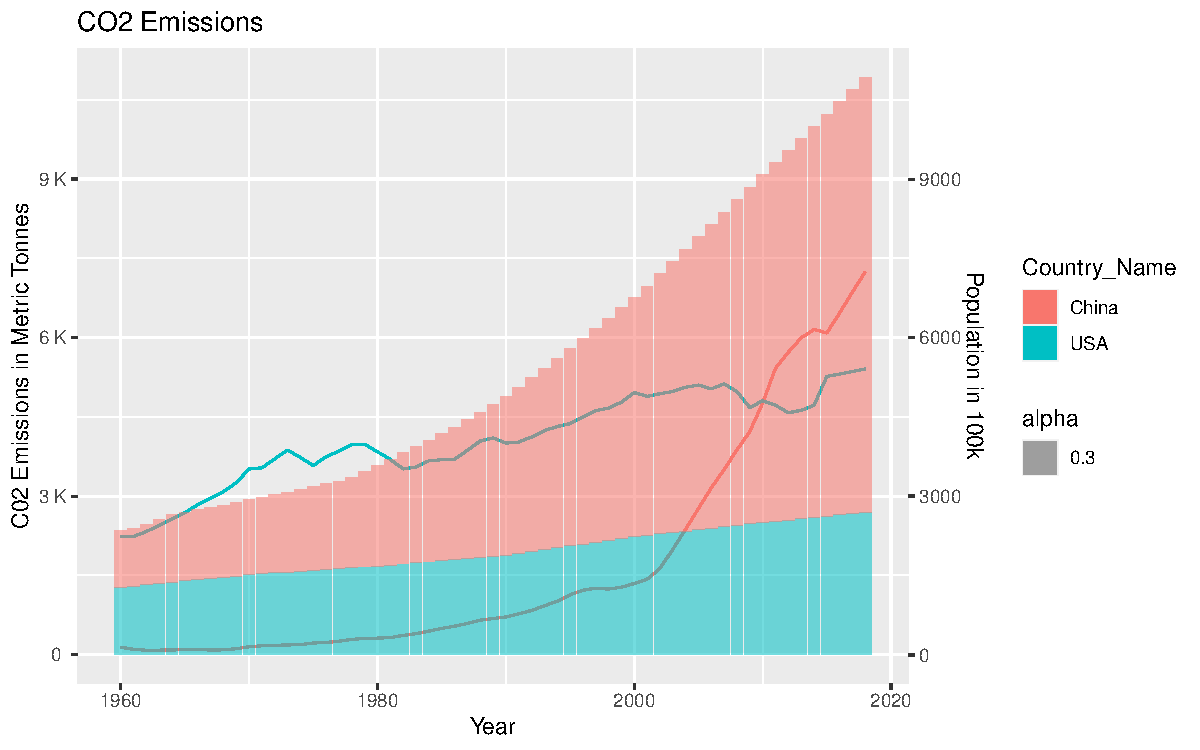
\includegraphics[width=7in, height = 2.5in]{Figures/total_carbon_emissions-1}
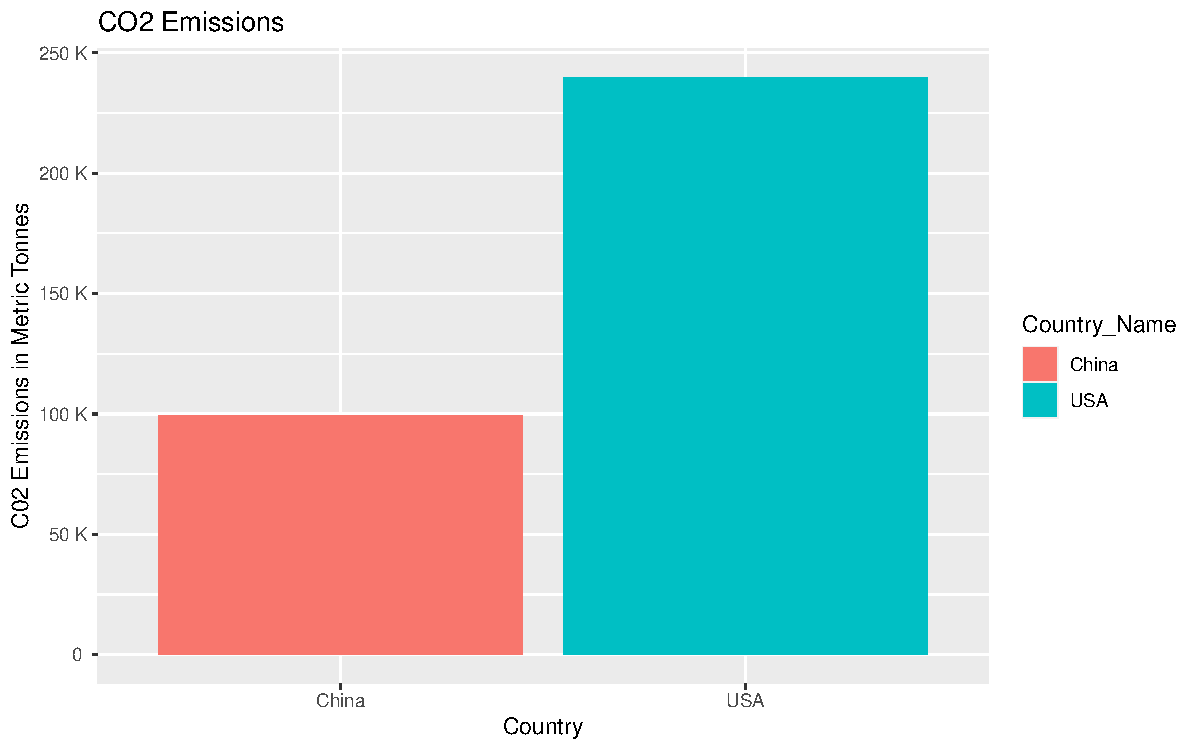
\includegraphics[width=7in, height = 2.5in]{Figures/total_carbon_emissions-2}
\caption{Total CO2 Emissions}
\label{fig:total_carbon_emissions}
\end{figure}

\begin{enumerate}
\def\labelenumi{\arabic{enumi})}
\setcounter{enumi}{1}
\tightlist
\item
  Research on the energy sources of each country and its impact and justify if per capita energy usage is an apt factor for comparision of these two countries. Which country has a better carbon footprint?
\end{enumerate}

Sustainable development has been recognized as an important goal by several countries. Emissions from sustainable sources such as biomass combustion are lower than fossil fuel combustion. Clean energy reduces environmental pollution, thus, improving public health, reducing premature mortality and saving on related health costs and will play a major role in combating climate change. The figure \ref{fig:energyusage_vs_co2emission} shows that CO2 emissions are proportional to the energy usage. The articles, \textcite{eia_US} and \textcite{eia_China}, show the energy distributions in both countries. It can be noted that China, though having lower per capita energy consumption contributes more to the carbon footprint that US, presently. This is because it is heavily dependent on coal whereas US has a higher dependence on natural gas, a clean energy source. Therefore, currently, US has a better carbon footprint.

The figure \ref{fig:proportion_countries_yearly} and the table \ref{tab:EnergyConsumptionComparision} show that the per capita energy consumption and CO2 emissions have been dominated severely by the US. The boxplot \ref{fig:distributionco2emissionenergyusageboxplot} shows that per capita energy usage and CO2 emission is higher for US in comparision to China. However, we know from above that it is due to the population difference between the two countries and China is considerably dependent on the non-clean energy sources. Therefore, scaling the energy usage and CO2 emission to per capita is not a correct measure to compare countries that have a huge population difference.

For more insights on the CO2 emissions from different countries, please refer \textcite{countriesC02emissions}.

\begin{figure}[H]
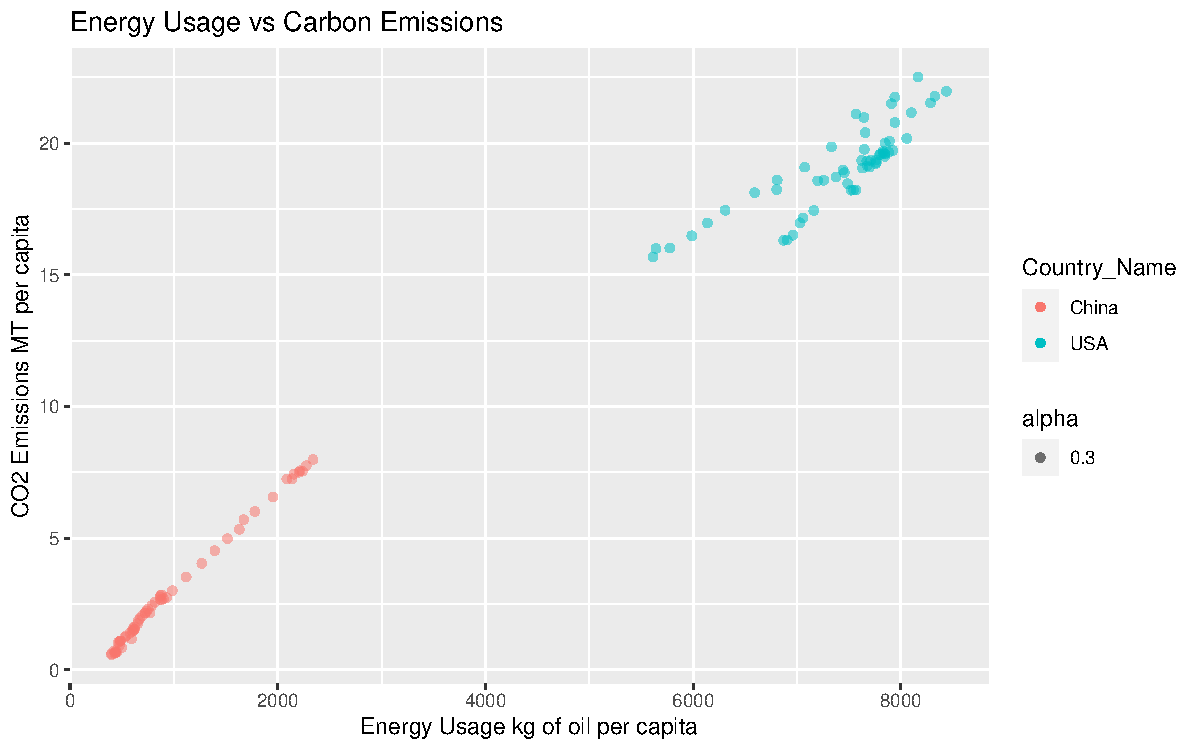
\includegraphics[width=7in, height = 2in]{Figures/energyusage_vs_co2emission-1}
\caption{Energy Usage vs Carbon Emissions}
\label{fig:energyusage_vs_co2emission}
\end{figure}

\begin{figure}[H]
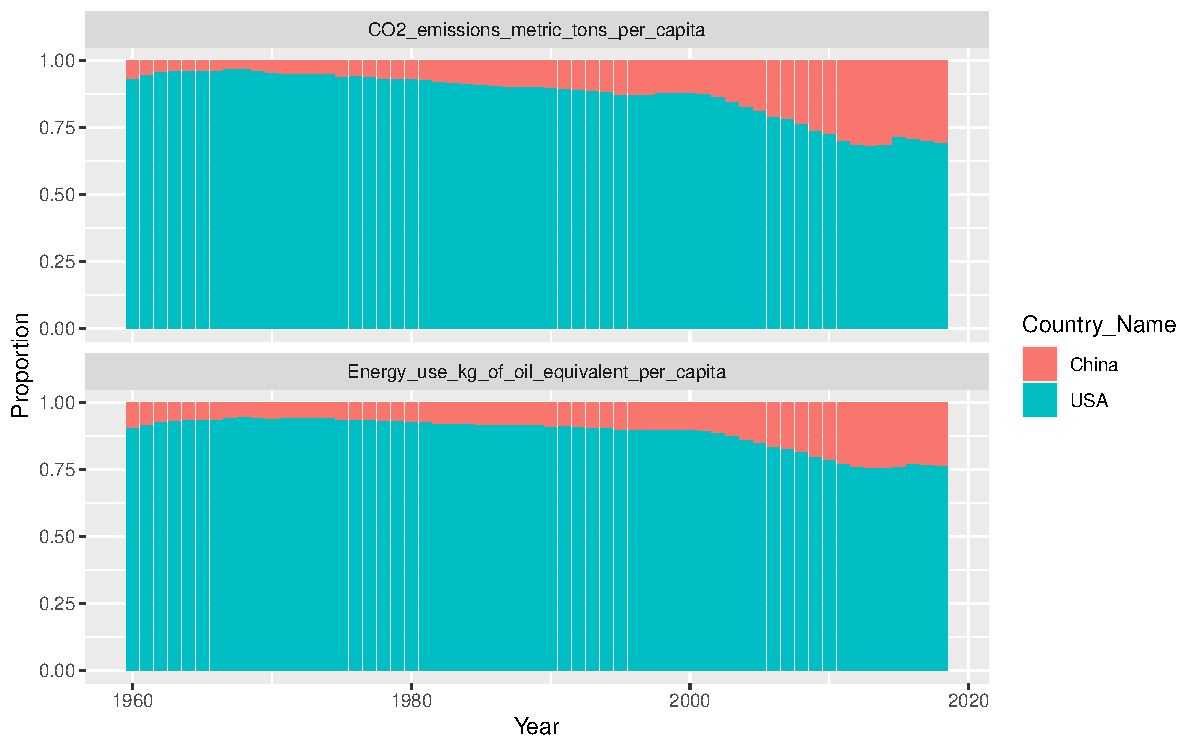
\includegraphics[width=6in, height = 2in]{Figures/proportion_countries_yearly-1}
\caption{Proportion Share Across The Years}
\label{fig:proportion_countries_yearly}
\end{figure}

\begin{figure}[H]
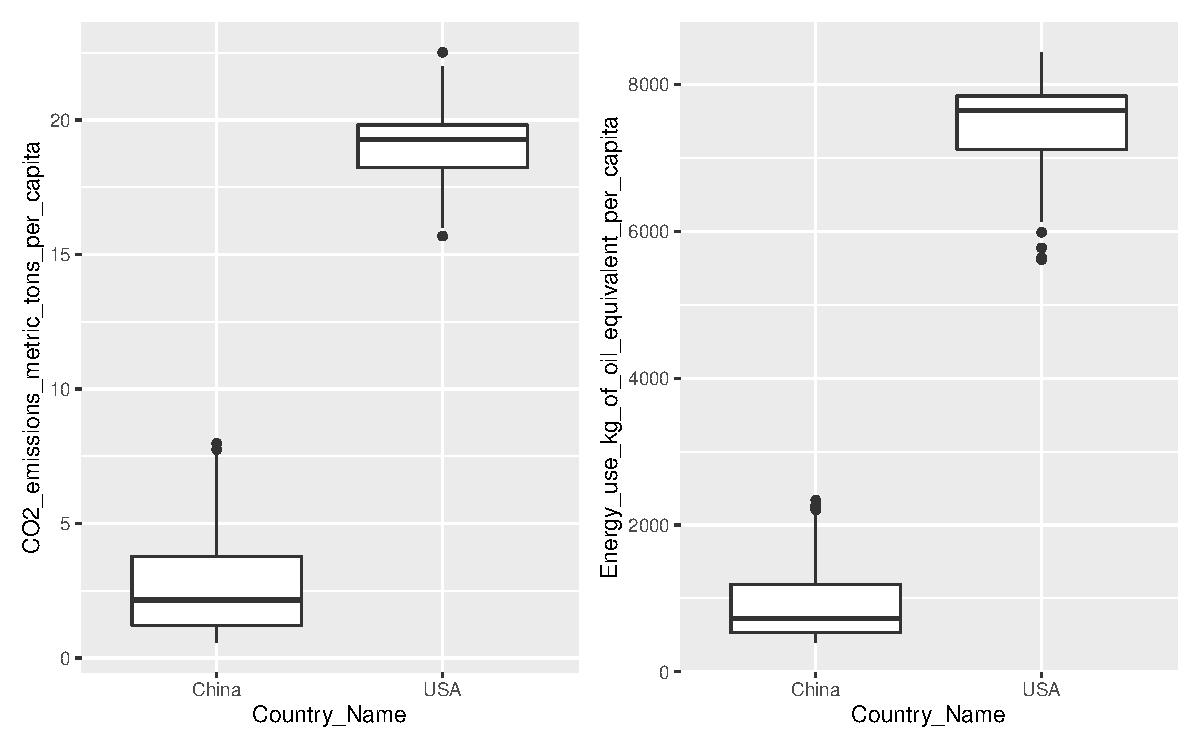
\includegraphics[width=7in, height = 3in]{Figures/distributionco2emissionenergyusageboxplot-1}
\caption{Distribution of CO2 Emissions and Energy Usage}
\label{fig:distributionco2emissionenergyusageboxplot}
\end{figure}

\begin{table}

\caption{\label{tab:EnergyConsumptionComparision}Energy Consumption Comparision}
\centering
\begin{tabular}[t]{r|r|r}
\hline
Year & USA & China\\
\hline
2018 & 7567.554 & 2338.658\\
\hline
2017 & 7543.050 & 2274.102\\
\hline
2016 & 7520.716 & 2204.976\\
\hline
2015 & 6803.919 & 2136.623\\
\hline
2014 & 6960.682 & 2236.730\\
\hline
2013 & 6905.647 & 2213.759\\
\hline
2012 & 6872.103 & 2155.165\\
\hline
2011 & 7030.033 & 2086.487\\
\hline
2010 & 7161.451 & 1954.723\\
\hline
2009 & 7056.784 & 1778.434\\
\hline
2008 & 7488.082 & 1672.904\\
\hline
\end{tabular}
\end{table}

\newpage
\subsection{Country Chile and Canada}

This section of the report focuses on the CO2 emissions(metric tonnes per capita) and energy usage(kg of oil equivalent per capita) for countries, Chile and Canada. The research questions addressed are the comparison of both countries on the basis of trend of CO2 emissions over the years and to determine which country has performed better with respect to CO2 emissions as well as energy usage.

Table analysis of both countries

\begin{table}[!h]

\caption{\label{tab:chile}CO2 Emissions of Chile}
\centering
\begin{tabular}[t]{l|l}
\hline
  & CO2\_emissions\_metric\_tons\_per\_capita\\
\hline
 & Min.   :1.659\\
\hline
 & 1st Qu.:2.069\\
\hline
 & Median :2.483\\
\hline
 & Mean   :2.823\\
\hline
 & 3rd Qu.:3.773\\
\hline
 & Max.   :4.736\\
\hline
 & NA's   :4\\
\hline
\end{tabular}
\end{table}

\begin{table}[!h]

\caption{\label{tab:canada}CO2 Emissions of Canada}
\centering
\begin{tabular}[t]{l|l}
\hline
  & CO2\_emissions\_metric\_tons\_per\_capita\\
\hline
 & Min.   :10.63\\
\hline
 & 1st Qu.:15.37\\
\hline
 & Median :16.31\\
\hline
 & Mean   :15.78\\
\hline
 & 3rd Qu.:17.02\\
\hline
 & Max.   :18.27\\
\hline
 & NA's   :4\\
\hline
\end{tabular}
\end{table}

It can be seen from table \ref{tab:chile}, that the mean CO2 emissions of Chile are 2.823 metric tons per capita while table \ref{tab:canada} shows Canada's mean CO2 emissions are 15.78 metric tons per capita. Both countries have a rising population but Chile has a better performance in terms of CO2 emissions.

Figure analysis of both countries

\begin{figure}

{\centering 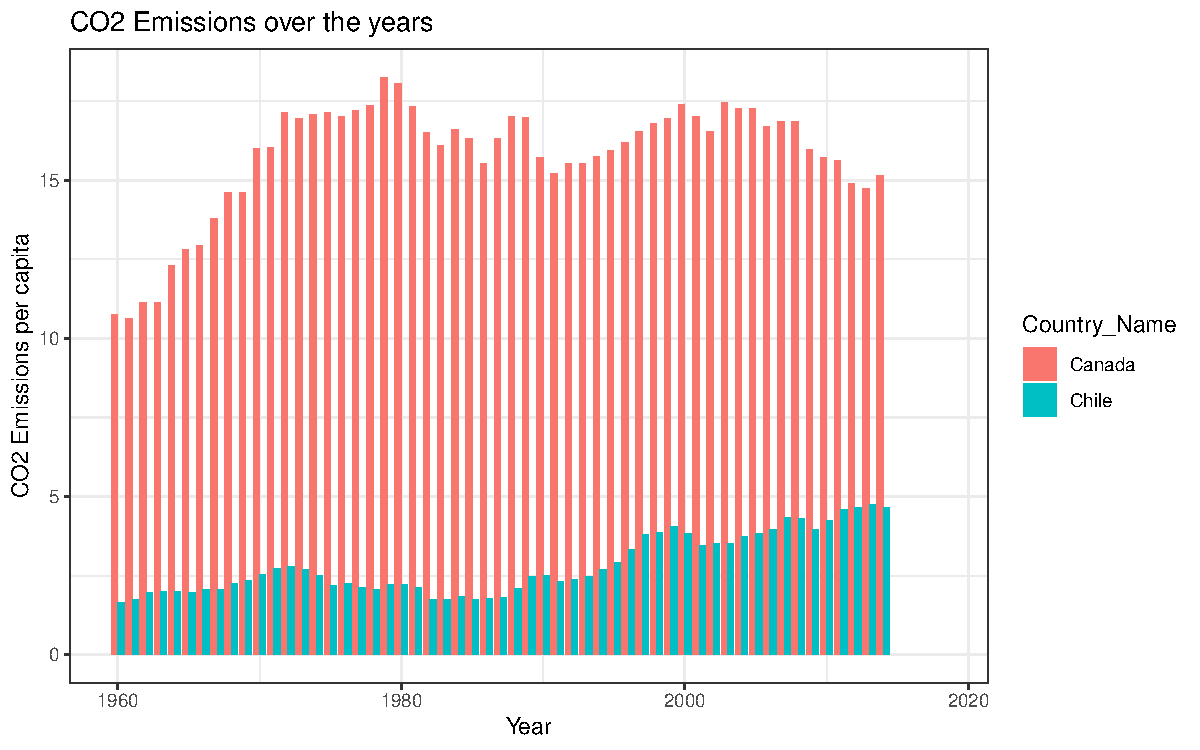
\includegraphics[width=0.5\linewidth]{Figures/emissions-1} 

}

\caption{CO2 Emissions over the years}\label{fig:emissions}
\end{figure}

The figure \ref{fig:emissions} represents the trend of CO2 emissions per capita of countries Chile and Canada.

\begin{figure}

{\centering 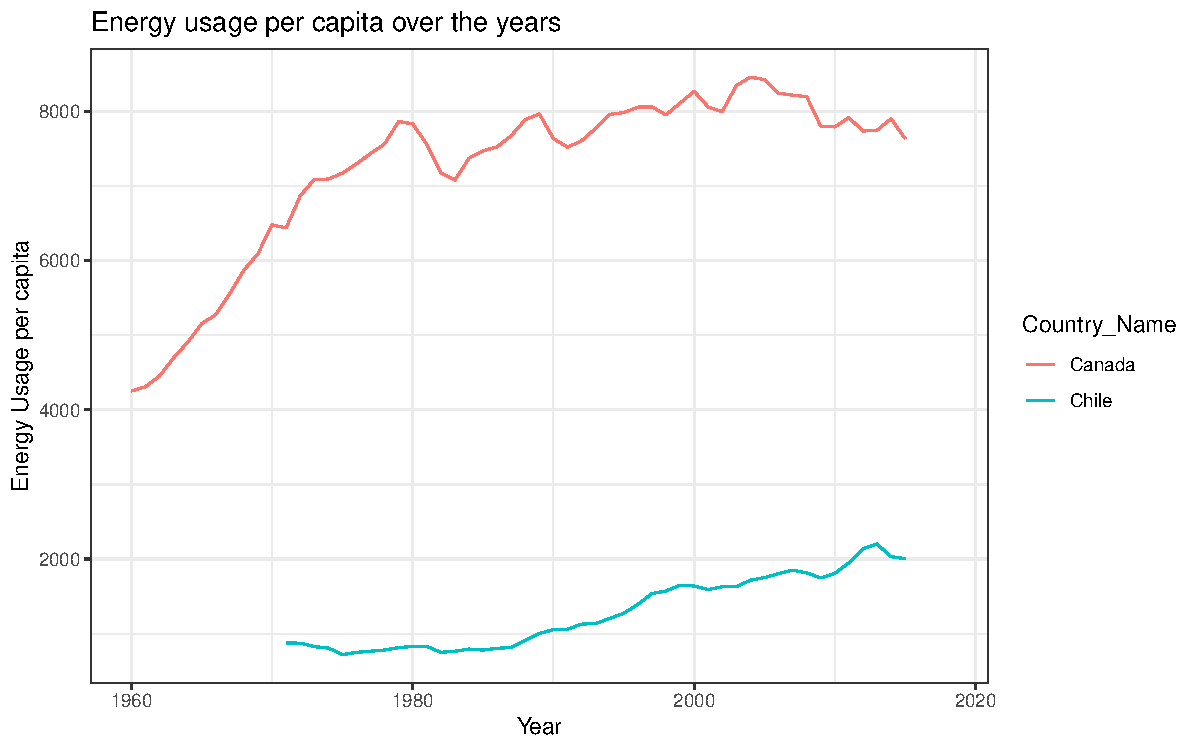
\includegraphics[width=0.5\linewidth]{Figures/energy-1} 

}

\caption{Energy usage per capita over the years}\label{fig:energy}
\end{figure}

The figure \ref{fig:energy} represents the trend of Energy usage per capita of countries Chile and Canada.

\begin{figure}

{\centering 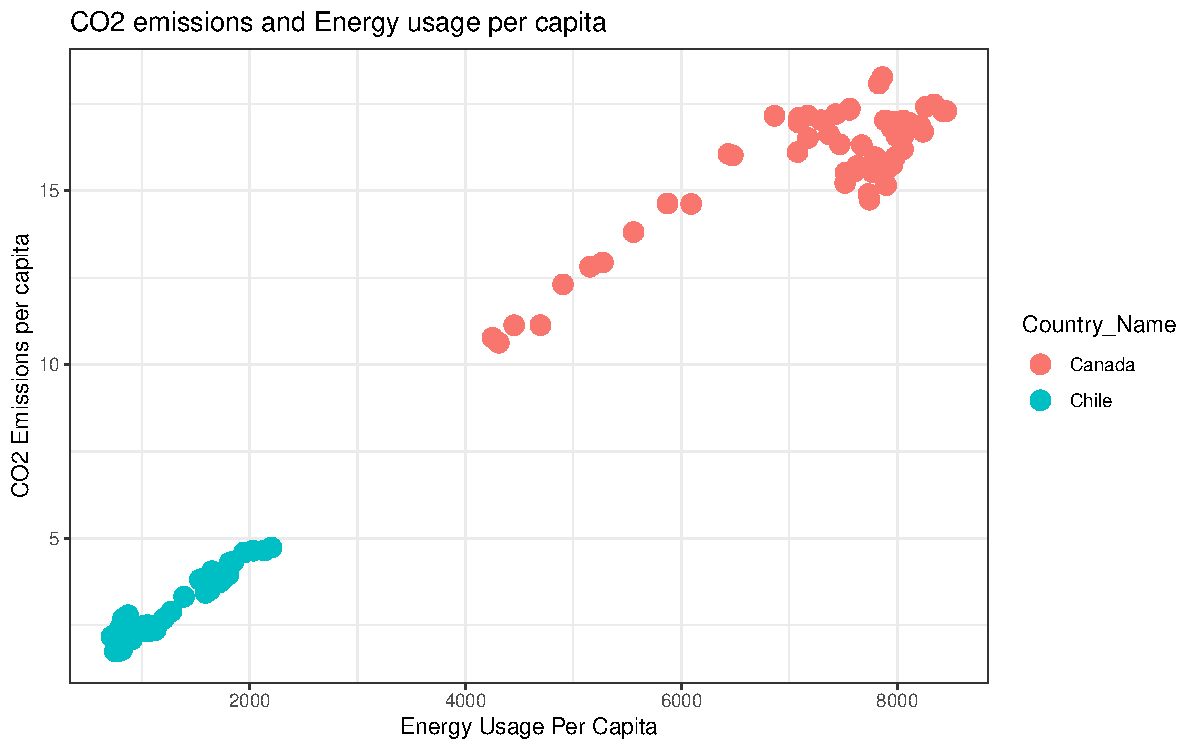
\includegraphics[width=0.5\linewidth]{Figures/plot-1} 

}

\caption{CO2 emissions and Energy usage per capita}\label{fig:plot}
\end{figure}

Figure \ref{fig:emissions} and Figure \ref{fig:energy} represent the trend of CO2 emissions and Energy usage per capita of Canada and Chile respectively. It can be observed that Chile has a better performance as it had less emissions and energy usage. Figure \ref{fig:plot} represents CO2 emissions and energy usage per capita of both countries.

To conclude, table \ref{tab:chile}, table \ref{tab:canada} and \ref{fig:emissions} represented the comparison of CO2 emissions in Chile and Canada, where Chile performed better. Figures \ref{fig:energy} and \ref{fig:plot} represented the overall measures of CO2 emissions and energy usage of both countries, where again Chile's measures were better. According to \textcite{joo2015energy}, the reason for CO2 emissions in Chile are because of its dependence on carbon energy consumption for its rising economic growth.

\subsection{Country United Arab Emirates and Singapore}

Table analysis

Table \ref{tab:uae} shows the mean per capita of co2 emission and energy use of United Arab Emirates is 30.6894 and 8639 respectively, and for Singapore, it is 9.6409 and 3838 as shown in Table \ref{tab:spg}. Although both countries are in high income group, Singapore has a better performance from the tables.

\begin{table}[!h]

\caption{\label{tab:uae}The summary of UAE}
\centering
\begin{tabular}[t]{l|l|l}
\hline
  & CO2\_emissions\_metric\_tons\_per\_capita & Energy\_use\_kg\_of\_oil\_equivalent\_per\_capita\\
\hline
 & Min.   :  0.1091 & Min.   : 2869\\
\hline
 & 1st Qu.: 19.0517 & 1st Qu.: 7209\\
\hline
 & Median : 28.7833 & Median : 9025\\
\hline
 & Mean   : 30.6894 & Mean   : 8639\\
\hline
 & 3rd Qu.: 35.8852 & 3rd Qu.:10972\\
\hline
 & Max.   :101.0517 & Max.   :12172\\
\hline
 & NA's   :4 & NA's   :15\\
\hline
\end{tabular}
\end{table}

\begin{table}[!h]

\caption{\label{tab:spg}The summary of SGP}
\centering
\begin{tabular}[t]{l|l|l}
\hline
  & CO2\_emissions\_metric\_tons\_per\_capita & Energy\_use\_kg\_of\_oil\_equivalent\_per\_capita\\
\hline
 & Min.   : 0.3488 & Min.   :1292\\
\hline
 & 1st Qu.: 7.0573 & 1st Qu.:2180\\
\hline
 & Median :10.9604 & Median :4423\\
\hline
 & Mean   : 9.6409 & Mean   :3838\\
\hline
 & 3rd Qu.:12.7502 & 3rd Qu.:5086\\
\hline
 & Max.   :18.0409 & Max.   :7371\\
\hline
 & NA's   :4 & NA's   :15\\
\hline
\end{tabular}
\end{table}

Figure analysis

In Figure \ref{fig:uae-sgp-co2-pop}, Singapore had stable C02 emissions of under 20 metric tons per capita with a growing population over years, while UAE fluctuated wildly with a higher average emissions. It was up to 101.0517 in 1969 with a low population, and fortunately kept dropping after that.

\begin{figure}[H]
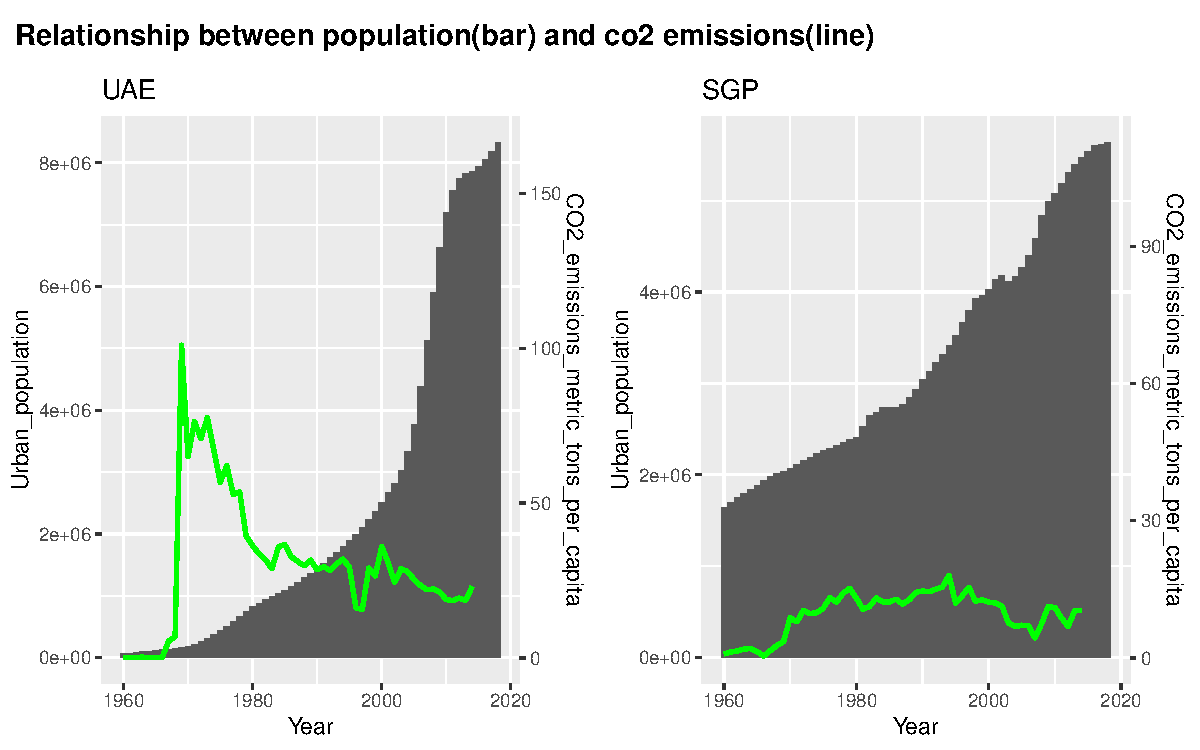
\includegraphics[width=7in, height = 4in]{Figures/uae-sgp-co2-pop-1}
\caption{population and co2 emissions relationship}
\label{fig:uae-sgp-co2-pop}
\end{figure}

In Figure \ref{fig:uae-sgp-energy-pop}, UAE has a higher energy use than Singapore and a smaller size of population. Increase and decrease sharply appears in both countries but the trend of Singapore is relatively less smooth than UAE's.

\begin{figure}[H]
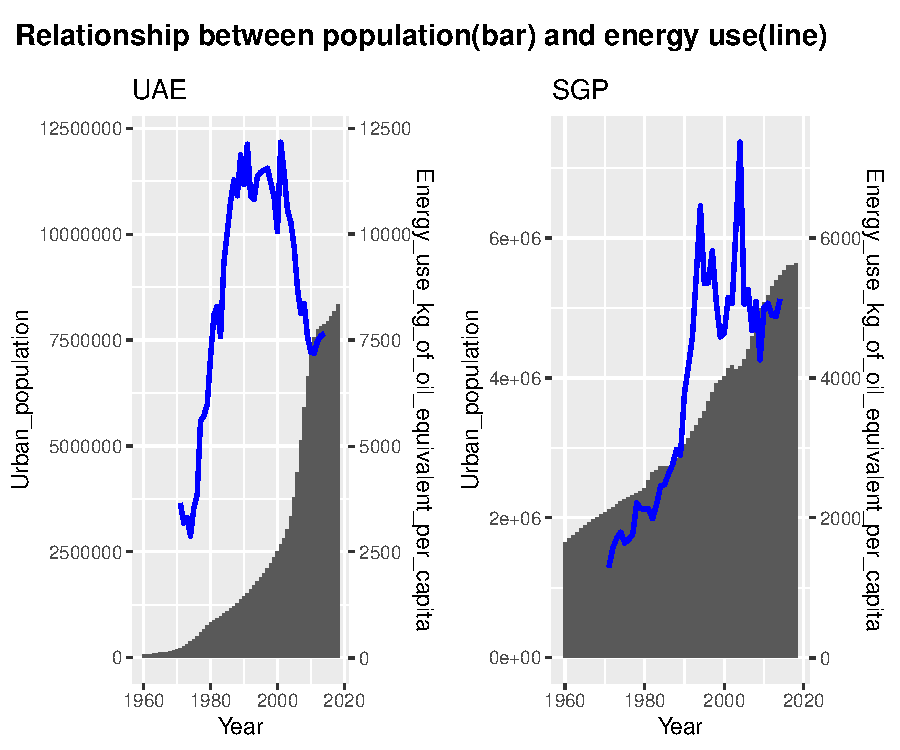
\includegraphics[width=7in, height = 3in]{Figures/uae-sgp-energy-pop-1}
\caption{population and energy use relationship}
\label{fig:uae-sgp-energy-pop}
\end{figure}

Both CO2 emissions and energy use trend of two countries will be discuss with the following figure.

\begin{figure}[H]
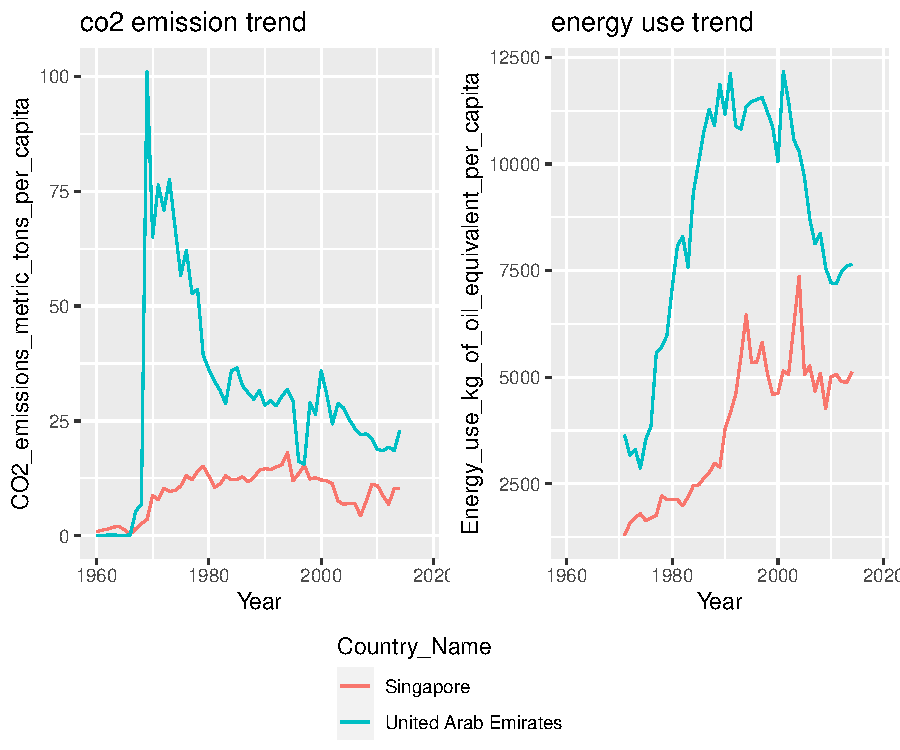
\includegraphics[width=7in, height = 4in]{Figures/uae-sgp-trend-1}
\caption{Trend of co2 emission and energy use}
\label{fig:uae-sgp-trend}
\end{figure}

The co2 emissions was up to 101.05 metric tons per capita in 1969, this might be due to oil commencmment of oil exports from 1962, and also the flight service operations in Dubai, especially for the private jets \textcite{reuters_2010}. From Figure \ref{fig:uae-sgp-trend}, Singapore performed better than UAE in either of the trend of CO2 emissions or energy usage as Singapore's trend is much smaller.

\addcontentsline{toc}{subsection}{Conclusion}
\subsection*{Conclusion}

In conclusion, all countries must gear up and implement strategies for climate action to make this world a better place. We say, save green, breathe pure, eat clean and live bonjour!!!

\newpage

\subsection*{R Packages}

\textcite{R-base}

\textcite{R-bookdown}
\textcite{R-citation}
\textcite{R-dplyr},

\textcite{R-forcats},

\textcite{R-ggplot2},

\textcite{R-kableExtra},

\textcite{R-knitr},

\textcite{R-naniar},

\textcite{R-patchwork},

\textcite{R-purrr},

\textcite{R-readr},

\textcite{R-scales},

\textcite{R-stringr},

\textcite{R-tibble},

\textcite{R-tidyr},

\textcite{R-tidyverse},

\textcite{R-tinytex},

\textcite{R-visdat},

\textcite{bookdown2016},

\textcite{ggplot22016},

\textcite{knitr2015},

\textcite{knitr2014},

\textcite{tidyverse2019},

\textcite{tinytex2019},

\textcite{visdat2017}

\printbibliography

\end{document}
